\section{Zielsetzung}
\label{sec:Zielsetzung}
Ziel dieses Versuches ist es den Brechungsindex von Silizium zu berechnen, indem die
Abhängigkeit der Intensität des an einem Silizium-Spiegel reflektierten Lichtes vom 
Eintrittswinkel und der Polarisation zu untersuchen.
\section{Theorie}
\label{sec:Theorie}
Das sich ausbreitende Licht wird in den meisten Fällen beim Durchqueren von Grenzflächen zweier
Medien mit zwei verschiedenen Brechungsindizes reflektiert und gebrochen. Dies wird in \autoref{fig:Abb_1} dargestellt.
\begin{figure}[H]
    \centering
    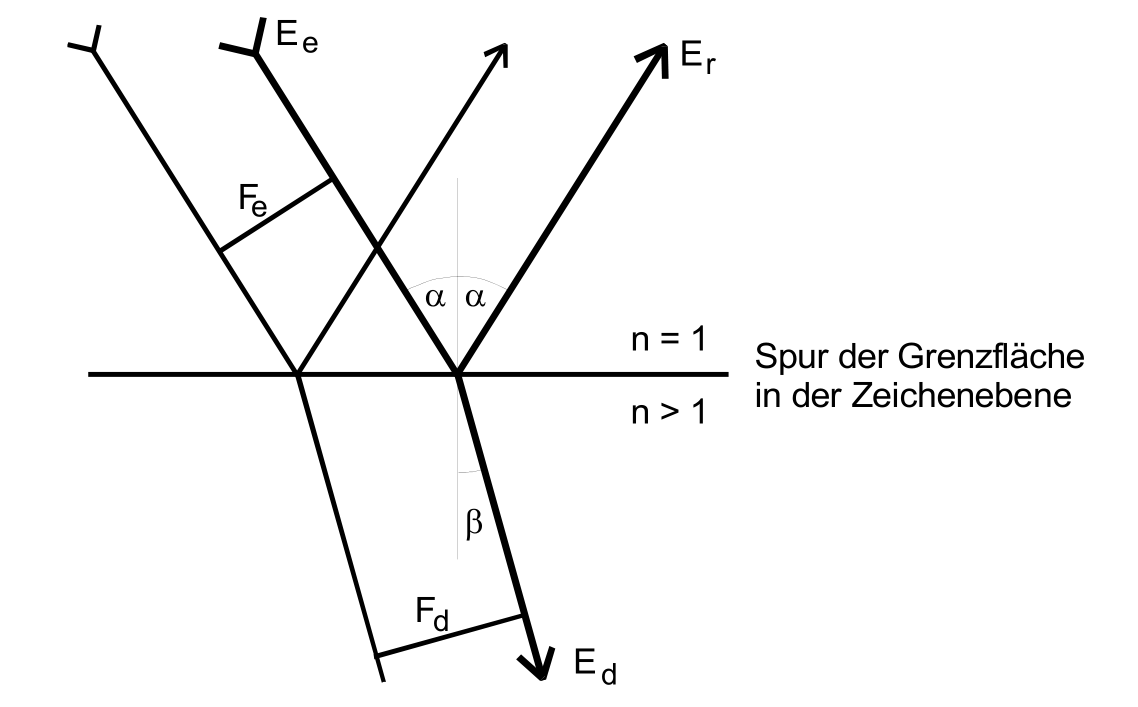
\includegraphics[width=0.5\textwidth]{Abbildung/Abb_1.png}
    \caption {Wechselwirkung eines Lichtstrahls an einer Grenzfläche \cite[42]{V407}.}
    \label{fig:Abb_1}
\end{figure}
Ein allgemeiner Ausdruck für die Strahlungsleistung von Lichtwellen wird benötigt um den Anteil zu bestimmen,
den das reflektierte und gebrochene Licht von der ursprünglichen Intensität besitzen.
Aus den Maxwell Gleichungen und der Elektrizitätslehre folgt der Poynting-Vektor
\begin{equation*}
    \vec{S} = \vec{E} \times \vec{H},
    \label{eqn:Poynting}
\end{equation*}
wobei $\vec{E}$ die elektrische und $\vec{H}$ die magnetische Feldstärke ist, welche eine
elektromagnetische Welle beschreibt. Der Poynting-Vektor beschreibt den Transport von Energie,
weil er in die Ausbreitungsrichtung der elektromagnetischen Welle zeigt und sein Betrag entspricht
der Energie der Strahlung. Er besitzt die Dimension $\frac{Leistung}{Fläche}$.\\
Trifft eine elektromagnetische Welle auf eine Grenzfläche teilt sich die Strahlungsleistung auf den 
reflektierten und gebrochen Teil auf. In diesem Versuch wird nur ein nicht absorbierendes Medium betrachtet,
weswegen für die Energieerhaltung
\begin{equation*}
    S_e \text{cos}(\alpha) = S_r \text{cos}(\alpha) + S_d \text{cos}(\beta)
\end{equation*}
gilt. Dabei bezeichnet $S_e$ den Betrag des Poynting-Vektors, also der einfallenden Strahlung und $S_r$ 
und $S_d$ analog die reflektierte und gebrochene Strahlung. Der einfallende Winkel wird durch 
$\alpha$ dargestellt und der Brechungswinkel wird durch $\beta$ dargestellt.
Mit den Winkeln und dem Snelliusschen Brechungsgesetz
\begin{equation*}
    n = \frac{\text{sin}(\alpha)}{\text{sin}(\beta)}
    \label{eqn:snellius}
\end{equation*}
lässt sich der Brechungsindex $n$ bestimmen, wobei außerdem 
\begin{equation}
    n = \frac{c}{v}
    \label{eqn:verhältnis}
\end{equation}
als Verhältnis der Geschwindigkeit von Licht in beiden Medien gilt.
Das Verhältnis zwischen reflektiertem und gebrochem Anteil der Strahlungsleistung ist
stark vom Polarisationszustand abhängig, daher müssen der senkrechte und parallel polarisierte
Strahlungsteil separat betrachtet werden. 
Für die senkrecht polarisierte Strahlung gilt
\begin{equation}
    \vec{E_{r\bot}}(\alpha) = \vec{E_{e\bot}} \frac{(\sqrt{n^2 - \text{sin}^2(\alpha)} - \text{cos}(\alpha))^2}{n^2 - 1}
    \label{eqn:senkrecht}
\end{equation}
und für die parallel polarisierte Strahlung gilt 
\begin{equation}
    \vec{E_{r||}}(\alpha) = \vec{E_{e||}} \frac{n^2 \text{cos}(\alpha) - \sqrt{n^2 - \text{sin}^2(\alpha)}}{n^2 \text{cos}(\alpha) + \sqrt{n^2 - \text{sin}^2(\alpha)}}
    \label{eqn:parallel}
\end{equation}
analog. Dabei ist $n$ der Brechungsindex und $\alpha$ der Winkel in dem die Strahlung auf die Gernzfläche trifft.
$\vec{E_r}$ und $\vec{E_e}$ sind die Amplituden der elektrischen Felder für den reflektierten und einfallenden Teil der 
Strahlung. Der Ausdruck für $\vec{E_{r||}}(\alpha)$ lässt sich auch als 
\begin{equation}
    \vec{E_{r||}}(\alpha) = \vec{E_{e||}}\frac{\text{tan}(\alpha - \beta)}{\text{tan}(\alpha + \beta)}
\end{equation}
schreiben, woraus folgt, dass $\vec{E_{r||}}(\alpha)$ null werden kann, wenn $\alpha + \beta = \qty{90}{\degree}$
erfüllt ist. $\vec{E_{r||}}(\alpha)$ verschwindet somit für einen bestimmten Winkel $\alpha$, sodass der gesamte reflektierte Anteil
und die gesamte Strahlung in das brechende Medium eindringt. Dieser Winkel ist der Brewsterwinkel, welcher durch die Relation
\begin{equation}
    \text{arctan}(n) =\alpha_B \label{eqn:brewster}
\end{equation}
ausgedrückt wird.